\section{Anweisungen}
	These der strukturierten Programmierung: 3 Anweisungen reichen aus, um jedes algorithmische Problem zu l�sen:
	\begin{compactitem}
  		\item Sequenz: Aufeinanderfolgende Anweisungen
  		\item Iteration: Die selbe Anweisung n-mal ausf�hren
  		\item Selektion: Anweisungen in Abh�ngigkeit einer Bedingung
  	\end{compactitem}
  	
	\subsection{Ausdrucksanweisungen}
    	\vspace*{-0.4cm}\begin{minipage}[t]{5 cm}
    		\subsubsection{Nullanweisung}  
   		 		Alleinstehender Strichpunkt   \\ 	
    			\lc{while(i < 5)\textbf{;}}    
    	\end{minipage}
    	\hspace*{0.5cm}
    	\begin{minipage}[t]{7 cm}
	    	\subsubsection{Zuweisung} 	    	
    			Einem Lvalue mittels \lc{=} , \lc{*=} , \lc{/=}, \lc{+=} oder \lc{-=} einen Wert zuweisen. \\   	
    			\lc{a=b=0 // entspricht a=(b=0)}
    	\end{minipage}	
   		\hspace*{0.5cm}
    	\begin{minipage}[t]{5 cm}
			\subsubsection{Funktionsaufruf} 
				\lc{getForFree(a, b);}
    	\end{minipage}
    	
	\subsection{Sprunganweisungen \verweisc{8.4}}
		Sprunganweisungen f�hren zu schlechtem Programmierstil und sollten nur in bestimmen F�llen eingesetzt werden, wie zum Bsp. \lc{break} bei \lc{switch}.
		\begin{compactitem}
			\item \lc{break}: \lc{do-while}-, \lc{while}-,  \lc{for}-Schleife und \lc{switch}-Anweisung abbrechen
			\item \lc{continue}: in den n�chsten Schleifendurchgang (Schleifenkopf) springen bei \lc{do-while}-, \lc{while}- und \lc{for}-Schleife 
			\item \lc{return}: aus Funktion an aufrufende Stelle zur�ckspringen mit R�ckgabe des Funktionswertes
			\item \lc{goto}: innerhalb einer Funktion an eine Marke (Label) springen
		\end{compactitem}
    	
	\begin{minipage}[t]{9 cm}
		\subsection{Sequenz \verweisc{8.1}}
			Die Sequenz ist eine zeitlich geordnete Abfolge von Anweisungen. \\
			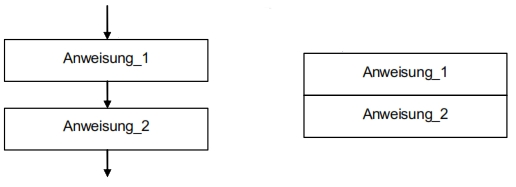
\includegraphics[width=1\textwidth]{pics/Sequenz.jpg}	
			
	\end{minipage}
	%
	\begin{minipage}[t]{9 cm}
			\subsubsection{Block}
				\begin{compactitem}
					\item Erfordert die Syntax genau eine Anweisung, so k�nnen dennoch mehrere Anweisungen geschrieben werden, wenn man sie in Form eines Blocks zusammenfasst.
					\item Ein Block wird mit geschweiften Klammern eingefasst. $\{ \dots \}$ Ein Block z�hlt syntaktisch als eine einzige Anweisung.
				\end{compactitem}
				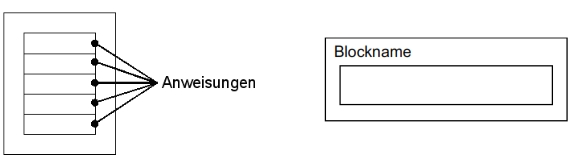
\includegraphics[width=1\textwidth]{pics/Block.jpg}
	\end{minipage}	   
    
	\subsection{Blockanweisungen}
		Anweisungen und Ausdr�cke innerhalb geschweifter Klammern. \\
    	\begin{minipage}[t]{9 cm}
        	\vspace*{-0.4cm}\lstinputlisting[language=C,tabsize=2]{code/block.c}
        \end{minipage}	
       	\hspace*{0.5cm}
        \begin{minipage}[t]{9 cm}
			Ausgabe: \\ \lc{x=15}  \lc{y=20} \\ \lc{x=5}  \lc{y=10} \\ kein Fehler, da der G�ltigkeitsbereich nur innerhalb des Blockes ist. Die ersten Variablen \lc{x} und \lc{y} werden im inneren Block lediglich �berdeckt.
        \end{minipage}
        
	\subsection{Selektionsanweisung \verweisc{8.2}}
		Von Selektion spricht man zum einen, wenn man eine Anweisung nur dann ausf�hren will, wenn eine bestimmte Bedingung zutrifft. Zum anderen m�chte man mit Selektionsanweisungen zwischen zwei M�glichkeiten (entweder/oder) bzw. zwischen mehreren M�glichkeiten genau eine ausw�hlen.
		
		\begin{minipage}[t]{5.5 cm}
			\subsubsection{Einfache Alternative}
				\lstinputlisting[language=C,tabsize=2]{code/strukturen_if_else.c}
		\end{minipage}
		%
		\begin{minipage}[t]{5.5 cm}
			\subsubsection{Bedingte Anweisung}
				\lstinputlisting[language=C,tabsize=2]{code/strukturen_if.c}
		\end{minipage}
		%
		\begin{minipage}[t]{7 cm}
			\subsubsection{Mehrfache Alternative - else if}
				\lstinputlisting[language=C,tabsize=2]{code/strukturen_else_if.c}
		\end{minipage}
		
		Wird innerhalb eines \lc{if} eine Variable deklariert, gilt sie bis zum Ende des \lc{if}.
		
		\subsubsection{Mehrfache Alternative - switch case}
			\begin{minipage}[t]{9 cm}
				
				\begin{compactitem}
					\item F�r eine Mehrfach-Selektion, d.h. eine Selektion unter mehreren Alternativen, kann die \lc{switch}-Anweisung verwendet werden, falls die Alternativen ganzzahligen Werten eines Ausdrucks von einem Integer-Typ entsprechen.
					\item Hat der Ausdruck der \lc{switch}-Anweisung den gleichen Wert wie einer der konstanten Ausdr�cke der \lc{case}-Marken, wird die Ausf�hrung des Programms mit der Anweisung hinter dieser \lc{case}-Marke weitergef�hrt.
					\item Stimmt keiner der konstanten Ausdr�cke mit dem \lc{switch}-Ausdruck �berein, wird zu \lc{default} gesprungen.
				\end{compactitem}							
			\end{minipage}
			\hspace*{1cm}
			\begin{minipage}[t]{9 cm}
				\vspace*{-0.5cm}
				\lstinputlisting[language=C,tabsize=2]{code/strukturen_switch.c}
			\end{minipage}
			
	\subsection{Iteration \verweisc{8.3}}
		\begin{minipage}[t]{4 cm}
			\vspace*{-0.4cm}\subsubsection{While}
				\vspace*{-0.4cm}\lstinputlisting[language=C,tabsize=2]{code/strukturen_while.c}			
		\end{minipage}
		\begin{minipage}[t]{14 cm}
			\vspace*{0.05cm}Schleifenrumpf wird ausgef�hrt solange Bedingung \lc{true} ergibt. \lc{do..while} und \lc{for} k�nnen grunds�tzlich aus \lc{while} gebaut werden.
		\end{minipage}
		
		\begin{minipage}[t]{10 cm}
			\subsubsection{For-Schleife}
				\vspace*{-0.4cm}\lstinputlisting[language=C,tabsize=2]{code/strukturen_for.c}
		\end{minipage}
		\begin{minipage}[t]{8 cm}
			\vspace*{0.45cm}Laufvariablen lokal deklarieren: \\\lc{for(int i=0; i<100; ++i)} \\Damit gilt sie nur innerhalb der Schleife.
		\end{minipage}

		\begin{minipage}[t]{4 cm}
			\subsubsection{Do-While}
				\vspace*{-0.4cm}\lstinputlisting[language=C,tabsize=2]{code/strukturen_dowhile.c}
		\end{minipage}
		\begin{minipage}[t]{14 cm}
			\vspace*{0.45cm}Schleifenrumpf wird mind. einmal ausgef�hrt und wiederholt falls Bedingung \lc{true} ergibt.
		\end{minipage}
		
		\subsubsection{Endlosschleife}
			\begin{minipage}[c]{3 cm}
				\vspace*{-0.4cm}\lstinputlisting[language=C,tabsize=2]{code/strukturen_endlos_for.c}
			\end{minipage}
			%
			\begin{minipage}[c]{3 cm}
				\vspace*{-0.4cm}\lstinputlisting[language=C,tabsize=2]{code/strukturen_endlos_while.c}
			\end{minipage}
		
		\subsubsection{Wann wird welche Schleife eingesetzt?}
			\begin{compactitem}
				\item For-Schleife: Bei Z�hlschleifen, d.h. wenn die Anzahl Durchl�ufe (kann auch variabel sein) im
				voraus feststeht.
				\item Do-While-Schleife: Wenn es keine Z�hlschleife ist, und die Schleife muss mindestens einmal
				durchlaufen werden
				\item While-Schleife: In allen anderen F�llen
			\end{compactitem}        